\section{Methodology}
\subsection{Simulation Procedure}
We introduce the overall simulation procedure to achieve our goal. The basic idea of the simulation is to verify and visualize the theories we used. We firstly set signal models to be used to measure waveform and signal strength. Path Loss, Gaussian white noise and Rayleigh fading are used in this step. Secondly, we design a model of robots that has a transmitter and receivers, and simulation field where the robots are placed and our algorithm are applied. Then we apply MUSIC algorithm to estimate the DOA.


\begin{figure}[ht]
	\centering
	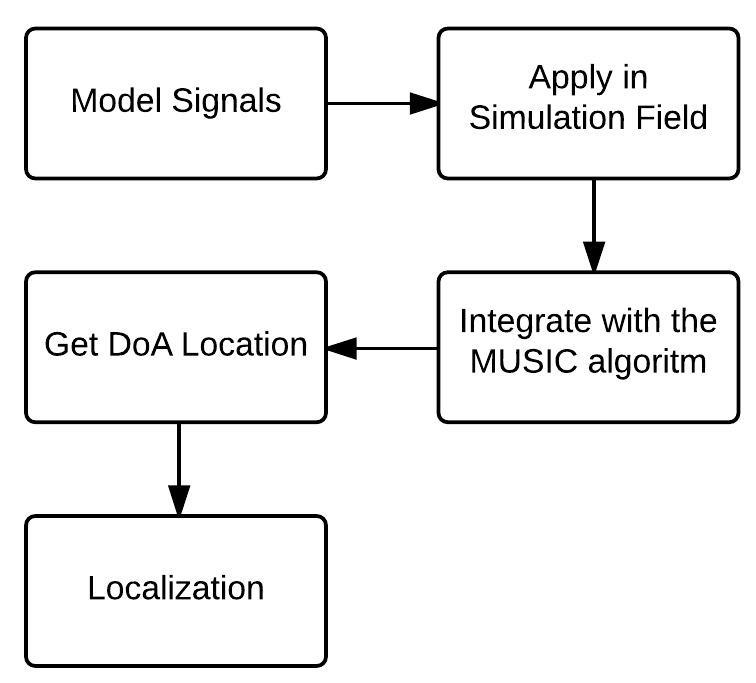
\includegraphics[width=0.4\textwidth]{procedure}
	\caption{Simulation Procedure}
	%\label{fig1}
	\end{figure}
	
The simulation is designed to see locations of robots and estimated distance by signal strength measured by robot's receivers. The location of the robots and some ranges from the robot are marked. The simulation assumes that field is a 2-D space that ranges 1000 meters by 1000 meters. The robots consist of a transmitter and four receivers with a interval of 0.6 meters. The marked range from robots are 200 meters and 100 meters and 20 meters representing the sensory range, the communication range and the rejection range respectively.



\begin{figure}[ht]
	\centering
	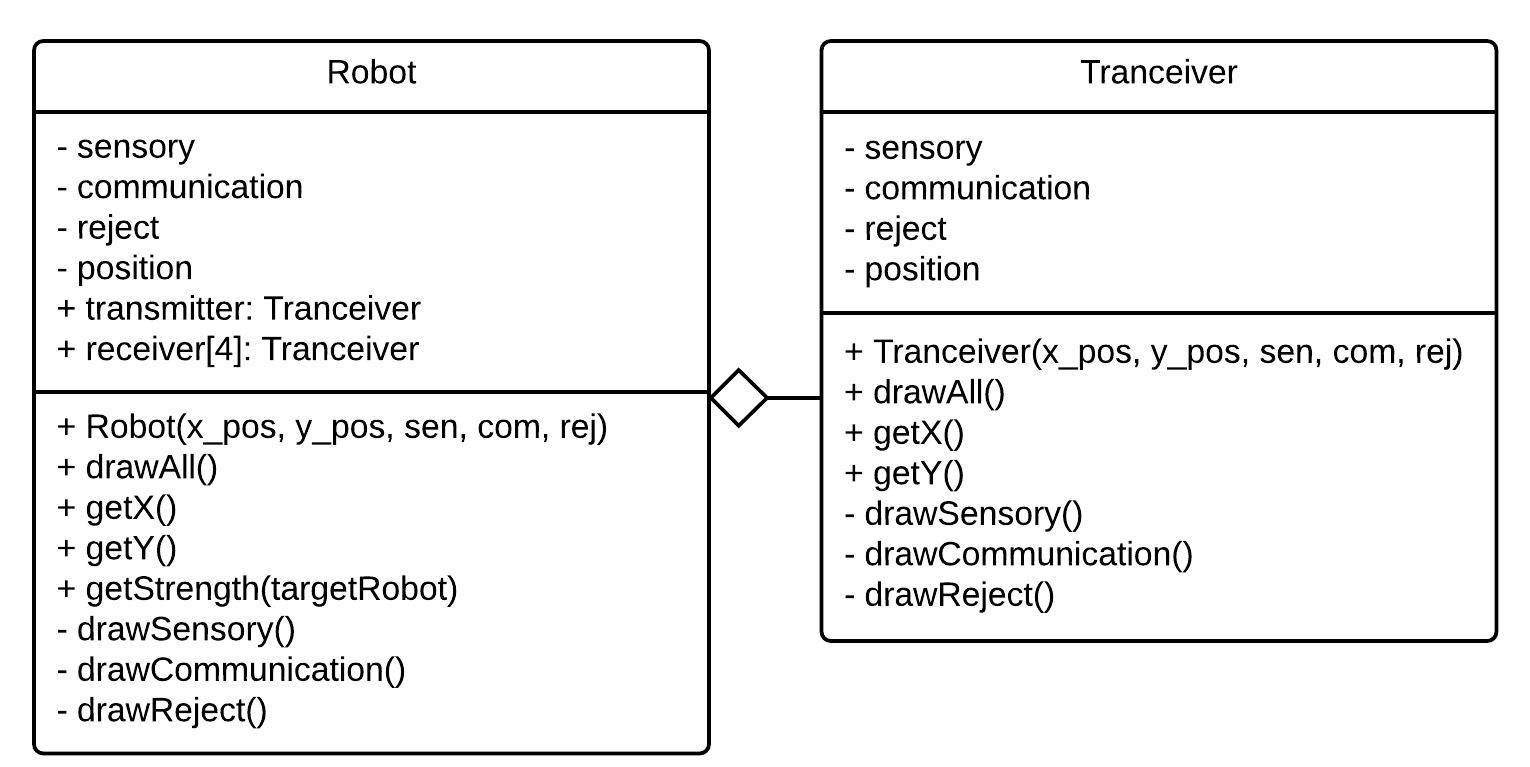
\includegraphics[width=0.4\textwidth]{classDiagram}
	\caption{Class Diagram of the simulation}
	%\label{fig1}
	\end{figure}
	

The simulation is written in MATLAB. The simulation consists of five files: 
\begin{itemize}
	\item simulation.m
	\item Robot.m
	\item Tranceiver.m
	\item simulation.m
	\item getSignalStrength.m
	\item drawCircle.m.
\end{itemize}

The drawCircle.m is used to draw circles on the simulation field to visualize the ranges of robots.

The getSignalStrength.m defines our signal model and accepts a distance value as an argument then returns a value of signal Strength. The model of signal will be discussed later.

Tranceiver.m defines the model of the signal transmitter and receiver using class. This class has four kinds of class member: sensory, communication, reject, and position. The class member sensory, communication, and reject are floating points in meters, representing those names of range. The class member position represents four antennas location of a robot.

Robot.m defines the class of the robot that has five instances of Tranceiver class:one is for transmitter and the other four are for receivers. This class has a method getStrength() that takes another instance of Robot and calculate signal strength between two robots. 

\begin{figure}[ht]
	\centering
	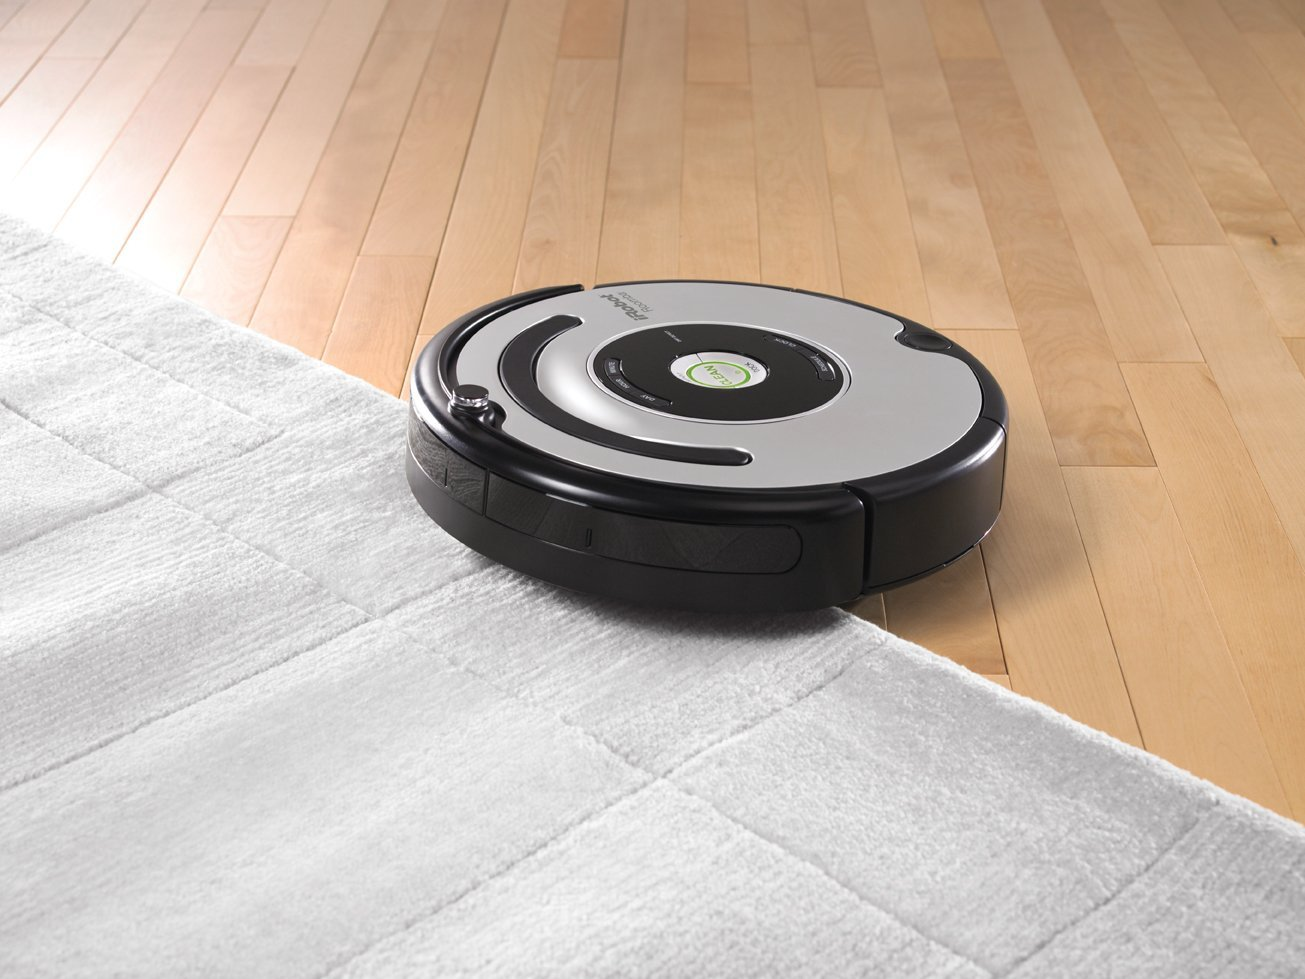
\includegraphics[width=0.5\textwidth]{RoombaTwo}
	\caption{Roomba}
	%\label{fig1}
	\end{figure}

\subsection{Signal Modelling}
In our signal modelling, we need to test the proper value of SNR, Rayleigh factor for our simulation. According to our test, the maximum proper value of Rayleigh factor is 0.0007 with 90\% (18 out of 20 cases) of success. A success means that all differences of every robot's true DOA and noised DOA are less than 45 degrees. Other values larger than 0.001 will decrease the success probability. This value can be lager as 0.0010 if we apply a low-pass filtered function to the signal. However, it will slow down our test speed, so we decide to use not filtered version of code as speed and cost trade-off. The minimum acceptable SNR is 34 with 90\%(18 out of 20 cases) success. SNR stands for signal noise ratio which will be explained later.
\par
	When we apply pmusic function to get DOA of each receiver robot from its transmitter robot, we can have the following table as reference:

\begin{table}[]
\centering
\label{Sample DOA data table}
\resizebox{0.4\textwidth}{!}{%
\begin{tabular}{|c|l|l|l|l|l|}
\hline
\multicolumn{2}{|l|}{} & \multicolumn{4}{c|}{{\color[HTML]{009901} \textbf{Transmmiter Robot}}} \\ \hline
{\color[HTML]{FE0000} } &  & {\color[HTML]{009901} \textbf{Robot1}} & {\color[HTML]{009901} \textbf{Robot2}} & {\color[HTML]{009901} \textbf{Robot3}} & {\color[HTML]{009901} \textbf{Robot4}} \\ \cline{2-6} 
{\color[HTML]{FE0000} } & {\color[HTML]{FE0000} \textbf{Robot1}} & 0 & 222.1875 & 23.9063 & 284.0625 \\ \cline{2-6} 
{\color[HTML]{FE0000} } & {\color[HTML]{FE0000} \textbf{Robot2}} & 56.2500 & 0 & 56.2500 & 57.6563 \\ \cline{2-6} 
{\color[HTML]{FE0000} } & {\color[HTML]{FE0000} \textbf{Robot3}} & 201.0938 & 305.1563 & 0 & 278.4375 \\ \cline{2-6} 
{\color[HTML]{FE0000} } & {\color[HTML]{FE0000} \textbf{Robot4}} & 146.2500 & 220.7813 & 81.5625 & 0 \\ \cline{2-6} 
{\color[HTML]{FE0000} } & {\color[HTML]{FE0000} \textbf{Robot5}} & 1.4062 & 286.8750 & 2.8125 & 333.2812 \\ \cline{2-6} 
{\color[HTML]{FE0000} } & {\color[HTML]{FE0000} \textbf{Robot6}} & 46.4062 & 257.3438 & 36.5625 & 341.7188 \\ \cline{2-6} 
{\color[HTML]{FE0000} } & {\color[HTML]{FE0000} \textbf{Robot7}} & 95.6250 & 250.3125 & 87.1875 & 30.9375 \\ \cline{2-6} 
{\color[HTML]{FE0000} } & {\color[HTML]{FE0000} \textbf{Robot8}} & 81.5625 & 33.7500 & 66.0938 & 64.6875 \\ \cline{2-6} 
{\color[HTML]{FE0000} } & {\color[HTML]{FE0000} \textbf{}} & {\color[HTML]{009901} \textbf{Robot5}} & {\color[HTML]{009901} \textbf{Robot6}} & {\color[HTML]{009901} \textbf{Robot7}} & {\color[HTML]{009901} \textbf{Robot8}} \\ \cline{2-6} 
{\color[HTML]{FE0000} } & {\color[HTML]{FE0000} \textbf{Robot1}} & 182.8125 & 234.8438 & 220.7813 & 229.2188 \\ \cline{2-6} 
{\color[HTML]{FE0000} } & {\color[HTML]{FE0000} \textbf{Robot2}} & 113.9062 & 102.6563 & 73.1250 & 187.0312 \\ \cline{2-6} 
{\color[HTML]{FE0000} } & {\color[HTML]{FE0000} \textbf{Robot3}} & 165.9375 & 227.8125 & 202.5000 & 255.9375 \\ \cline{2-6} 
{\color[HTML]{FE0000} } & {\color[HTML]{FE0000} \textbf{Robot4}} & 106.8750 & 135.0000 & 229.2188 & 210.9375 \\ \cline{2-6} 
{\color[HTML]{FE0000} } & {\color[HTML]{FE0000} \textbf{Robot5}} & 0 & 329.0625 & 302.3438 & 284.0625 \\ \cline{2-6} 
{\color[HTML]{FE0000} } & {\color[HTML]{FE0000} \textbf{Robot6}} & 135.0000 & 0 & 347.3437 & 282.6563 \\ \cline{2-6} 
{\color[HTML]{FE0000} } & {\color[HTML]{FE0000} \textbf{Robot7}} & 130.7813 & 32.3437 & 0 & 188.4375 \\ \cline{2-6} 
\multirow{-18}{*}{{\color[HTML]{FE0000} \textbf{\begin{tabular}[c]{@{}c@{}}Receiver\\ Robot\end{tabular}}}} & {\color[HTML]{FE0000} \textbf{Robot8}} & 85.7813 & 108.2812 & 12.6563 & 0 \\ \hline
\end{tabular}%
}
\caption{Numbers are DOA represented in degrees. 0 means robot is receiving its own signal.}
\end{table}


\subsection{Formula}
The equation of path loss is:
\begin{equation}
L(d)=10*n*log_{10}d + C
\end{equation}
where $L$ is the path loss in decibels, $n$ is the path loss exponent, $d$ is the distance between the transmitter and the receiver, usually measured in meters, and $C$ is a constant which accounts for system losses.
\par
In our model, we use a reference distance and signal strength to get the signal strength:
\begin{equation}
p_{L}(d)=L(d_{0})-20log_{10}(d/d_{0})
\end{equation}
where $d_{0}$ is the reference distance of an antenna, $L(d_{0})$ is the signal strength at $d_{0}$. The value of $d_{0}$ and $L(d_{0})$ depends on characteristic of an antenna.
\\
\vspace{1cm}

The Gaussian White Noise has the probability density function $p_{G}$ of a normal distribution with random variable $x$ in our case is:
\begin{equation}
p_{G}(x)={\frac {1}{ {\sigma\sqrt {2\pi }}}}e^{-{\frac {x^{2}}{2\sigma}}}
\end{equation}
where $\sigma$  the standard deviation. The standard deviation in our model depends on performance of antenna, which can be represented as Signal-to-Noise Ratio (SNR).
\vspace{1cm}

The Rayleigh fading is the effect when there are objects like wall in the field that scatter the radio signal. The Rayleigh fading has a model with Rayleigh distributed probability density function, that is:
\begin{equation}
p_{R}(r)={\frac {2r}{\Omega }}e^{-r^{2}/\Omega },\ r\geq {}0
\end{equation}
where $R$ is random variable, and $\Omega$ is the mean value of square of $r$: $\Omega = E(R^{2})$.
\vspace{1cm}

To sum up, the received signal strength of the receiver antenna is:
\begin{equation}
p(d)=p_{L}(d)+p_{G}(x)+p_{R}(r)
\end{equation}
where $L(d)$ is the path loss, $p_{G}(x)$ is the Gaussian White Noise, and $p_{R}(r)$ is the Rayleigh fading.
\vspace{1cm}



If $\mathbf{v}_i$ are the noise eigenvectors and
\begin{equation}
\mathbf{e} = \begin{bmatrix}1 & e^{j \omega} & e^{j 2 \omega} & \cdots & e^{j (M-1) \omega}\end{bmatrix}^T.
\end{equation}
Then the frequency estimation function for MUSIC is:
\begin{equation}
\hat P_{MU}(e^{j \omega}) = \frac{1}{\sum_{i=p+1}^{M} |\mathbf{e}^{H} \mathbf{v}_i|^2},
\end{equation}
\begin{figure}[ht]
	\centering
	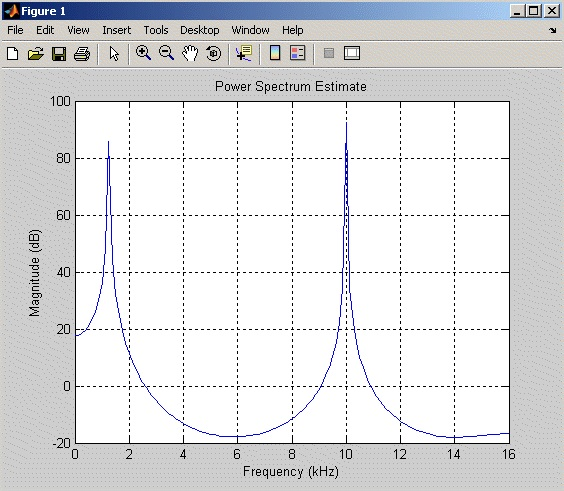
\includegraphics[width=0.4\textwidth]{MusicGraph}
	\caption{Power Spectrum Using MUSIC}
	%\label{fig1}s
	\end{figure}
Spectral density estimation is to estimate the spectral density of a random signal from a sequence of time samples of the signal. In our case, the maximum value of $hat P_{MU}$ converted to degrees is the DOA of robots.
%\begin{figure}[h]
%\centering
%\includegraphics[width=0.8\linewidth]{img/img1}
%\caption{3D terrain surface}
%\label{fig4}
%\end{figure} 